\documentclass[a4paper]{article}

\usepackage[french]{babel}
\usepackage[utf8]{inputenc}
\usepackage{graphicx}
\usepackage{pdfpages}

\title{SmallWorld : Documentation utilisateur \\ INSA de Rennes - 4INFO}

\author{Axel CARO, Maximilien RICHER}

\date{\today}

\begin{document}
\maketitle

\tableofcontents

\newpage

\section*{Introduction}
\paragraph{}
Ce jeu vidéo est basé sur le jeu de plateau \textit{SmallWorld}. Il s'agit donc d'un jeu en tour par tour.
Au cours d'une partie, les joueurs s'affrontent pendant un certain nombre de tours afin de prendre le contrôle d'un territoire.

\section{Présentation des règles du jeu}

\subsection{But du jeu}
\paragraph{}
Le but de SmallWorld est d'accumuler des points de victoire.
À la fin de chaque tour de jeu, le joueur compte les points gagnés et les ajoute à son total. Au bout d'un nombre de tour défini au préalable, le jeu s'arrête et le joueur ayant le plus de points remporte la partie. Une partie peut également s'interrompre si un des joueurs élimine l'ensemble des unités de l'adversaire. Un joueur qui ne possède plus d'unités perd la partie, quel que soit son total de point.

\paragraph{}
\textbf{Déroulement d'une partie : }
\begin{itemize}
    \item Choix de la configuration du plateau de jeu
    \item Choix des races
    \item Création du plateau de jeu
    \item Début du premier tour de jeu\\(\dots)
    \item Fin du dernier tour de jeu
    \item Décompte final des points
\end{itemize}

\subsubsection{Plateau de jeu}
\paragraph{}
Le jeu se déroule sur un plateau quadrillé de cases carrées dont la dimension dépend principalement de la durée de la partie (nombre de tours).\label{map_gen} Il est composé de cases de différents types : plaine, mer, montagne et forêt. La carte est générée de manière aléatoire, mais doit contenir le même nombre de cases de chaque type.

\subsubsection{Unités}
\paragraph{}
Des unités sont placées sur le plateau, sur lequel elles peuvent être déplacées. Elles possèdent des points d'action, rechargés en début de tour, mais aussi une jauge de vie et des statistiques d'attaque et de défense.

\subsubsection{Races et décompte des points en fin de tour}
À la fin de chaque tour, le joueur compte les points gagnés et les ajoute à son total. Le montant des points gagnés est déterminé en fonction de la race choisie et du type de terrain sur lequel ses unités sont placées.

\paragraph{}
\textbf{Configurations conseillées :}
\begin{itemize}
    \item 2 joueurs, plateau de 6 par 6, 5 tours de jeu : 4 unités par joueur
    \item 2 joueurs, plateau de 10 par 10, 20 tours de jeu : 6 unités par joueur
    \item 2 joueurs, plateau de 14 par 14, 30 tours de jeu : 8 unités par joueur
\end{itemize}

\subsection{Déroulement d'un tour de jeu}
\paragraph{}
Chaque \textit{tour de jeu} est constitué de plusieurs \textit{tours de joueurs}. Ces tours sont séquentiels. Lors du premier tour de jeu, le joueur jouant le premier tour est tiré au hasard, et cet ordre est conservé durant le reste de la partie.

\paragraph{}
\textbf{Déroulement du tour : }
\begin{itemize}
    \item Début du tour
    \item Déplacement des unités et combats
    \item Décompte des points
    \item Fin du tour
\end{itemize}

\subsection{Déplacement et combat}
\paragraph{}
Un joueur peut, durant son tour, déplacer une ou plusieurs unités lui appartenant. Une unité ne peut être déplacée que s'il lui reste assez de points d'action pour effectuer le déplacement demandé. Le nombre de points d'action nécessaires dépend de la race du joueur et du type des cases traversées. Les déplacements ne peuvent s'effectuer que vers une case adjacente, et non en diagonale. Un déplacement vers une case occupée par une ou plusieurs unités alliées est autorisé. Un déplacement vers une case occupée par une unité adverse engendre un combat.

\paragraph{}
Il est possible d'attaquer une unité plusieurs fois de suite, à condition de disposer des points d'action nécessaires.

\subsubsection{Combat au corps à corps}
Le combat au corps à corps est provoqué par un déplacement. Dans le cas de la mort de l'unité adverse, l'attaquant est déplacé sur sa case si aucune autre unité adverse ne s'y trouve encore. Dans le cas contraire, il conserve sa position.
\subsubsection{Combat à distance}
Un combat à distance n'implique pas de déplacement. L'attaquant doit se trouver sur la même ligne ou la même colonne que sa cible, à deux cases de distance (boir \ref{range}. Sur la case vide situé entre l'attaquant et sa cible peut se trouver une unité allié ou adverse sans que cela n'ai d'incidence sur le déroulement de l'attaque.
Contrairement à l'attaque au corps à corps, aucun déplacement n'est généré en cas de décès du défenseur.

\begin{figure}[h]
\begin{center}
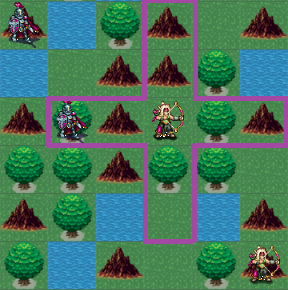
\includegraphics[scale=0.7]{./img/range_arrow.png}
\caption{\label{range}Portée d'un combattant à distance}
\end{center}
\end{figure}

\newpage
\section{Installation de l'application}
\paragraph{}
Le jeux se présente sous la forme d'un ficher d'archive zip à décompresser. Il est prévu pour fonctionner sur Windows 7/8.1/10 en version i386 ou x64.

\section{Démarrer une partie}
\paragraph{}
Après avoir lancé l'exécutable, vous arrivez devant l'écran de lancement du jeu. Celui-ci vous permet d’effectuer divers réglages, notamment :

\begin{itemize}
    \item Choisir les pseudonymes des joueurs
    \item Régler la taille de la carte
    \item Choisir la race de chaque joueur
    \item Charger une sauvegarde existante
\end{itemize}


\begin{figure}[h]
\begin{center}
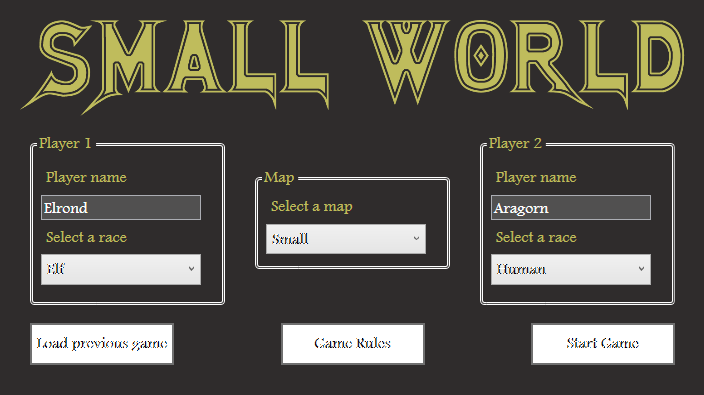
\includegraphics[scale=0.4]{./img/start_screen.png}
\caption{L'écran de lancement du jeu}
\end{center}
\end{figure}

\begin{figure}[h]
\begin{center}
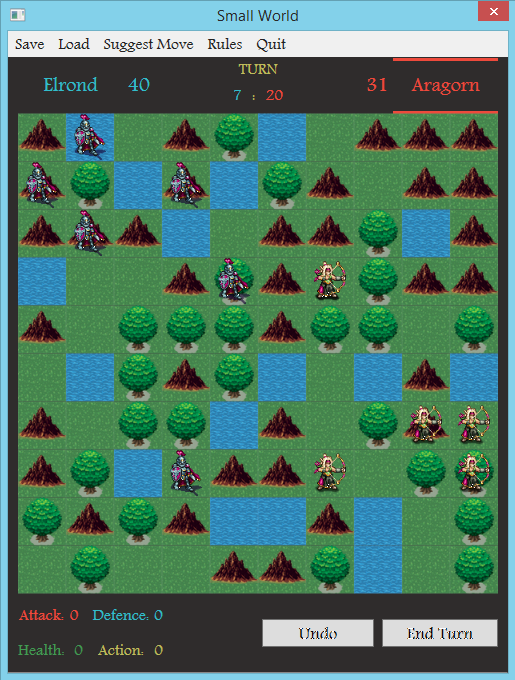
\includegraphics[scale=0.5]{./img/game_window.png}
\caption{Une partie de Small World}
\end{center}
\end{figure}

\section{Commandes}
\paragraph{}

\begin{tabular}{|l|c|}
  \hline
  Action & Commande \\
  \hline
  Sélectionner & Clic gauche sur l'unité \\
  Déplacer & Clic droit sur la case de destination \\
  Attaquer & Clic droit sur l'unité cible \\
  Sauvegarder une partie & Menu: Save \\
  Charger une partie & Menu: Load \\
  Annuler une action & Bouton: Undo \\
  Fin de tour & Bouton: End Turn \\
  \hline
\end{tabular}
\newpage
\section{Trucs et astuces}

\subsection{Fenêtre de log}
\paragraph{}
À chaque action effectuée, une description des évènements est affichée dans la fenêtre de log. Ceci prend en compte les déplacements, les affrontements, et les débuts et fins de tours.

\subsection{Suggestion de mouvements}
\paragraph{}
Si vous ne savez pas quoi jouer ce tour-ci, le jeu peut vous suggérer des mouvements possibles. Sélectionnez une unité puis appuyer sur \textit{Suggest Move}. Les cases suggérées deviendrons rouges.

\begin{figure}[h]
\begin{center}
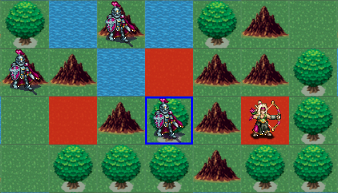
\includegraphics[scale=0.4]{./img/suggest_move.png}
\caption{Suggestion de mouvement}
\end{center}
\end{figure}

\subsection{Règles détaillées}
\paragraph{}
Vous pouvez accéder à une aide en jeu à tout moment via le bouton \textit{Game Rules}.

\begin{figure}[h]
\begin{center}
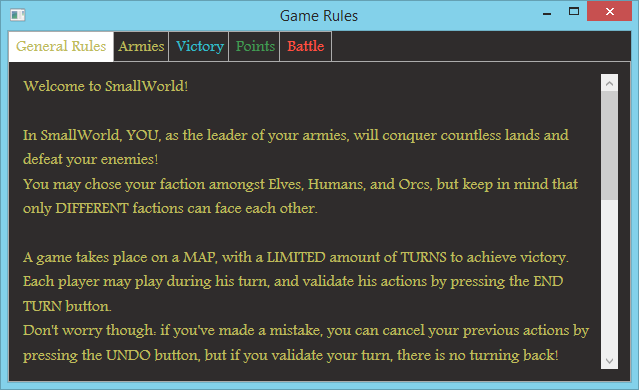
\includegraphics[scale=0.52]{./img/help.png}
\caption{Aide en jeu}
\end{center}
\end{figure}


\end{document}